\chapterstyle{texto}


\chapter{Resultados Preliminares} 
\label{resultados_preliminares}

\section{Índices de Sentimento}

Foram produzidas oito variações do índice de sentimento para a política monetária fruto da combinação entre os quatro dicionários de polaridade e as duas fórmulas de agregação de sentimento. Os melhores resultados em termos de significância estatística nos modelos VAR e \textit{Local Projections} vieram dos índices baseados na fórmula de agregação utilizada em \textcite{carosia_analyzing_2020} e, particularmente, do dicionário SentiLex. 

Devido à intensa volatilidade dos indicadores, a visualização múltipla em uma única figura se torna inviável. Não obstante, a fim de visualizar e, possivelmente, identificar algum comportamento geral entre os índices optou-se por empregar a método de Análise de Componentes Principais (PCA). Esse procedimento permite reduzir a dimensionalidade dos dados, extraindo camadas ortogonais (os componentes principais), que explicam a maior parte da variação dos dados.

A Figura \ref{graf:pca} mostra a evolução do Componente Principal extraído dos índices de sentimento baseado na fórmula de agregação de  \textcite{carosia_analyzing_2020}. Foi plotado ainda, em área sombreada, o intervalo entre os valores mínimos e máximos dos índices de sentimento do qual o componente principal foi extraído. A escala de valores foi normalizada de maneira que a unidade represente um desvio-padrão. Algumas datas importantes em termos de política monetária foram destacadas por linhas verticais, bem como os quatro valores máximos e mínimos do indicador.  

\begin{figure}[H]
    \captionsetup{position=above} % Puts the caption above the image
    \caption{Componente Principal e intervalo de máximos e mínimos de quatro índices de sentimento}
    \centering
    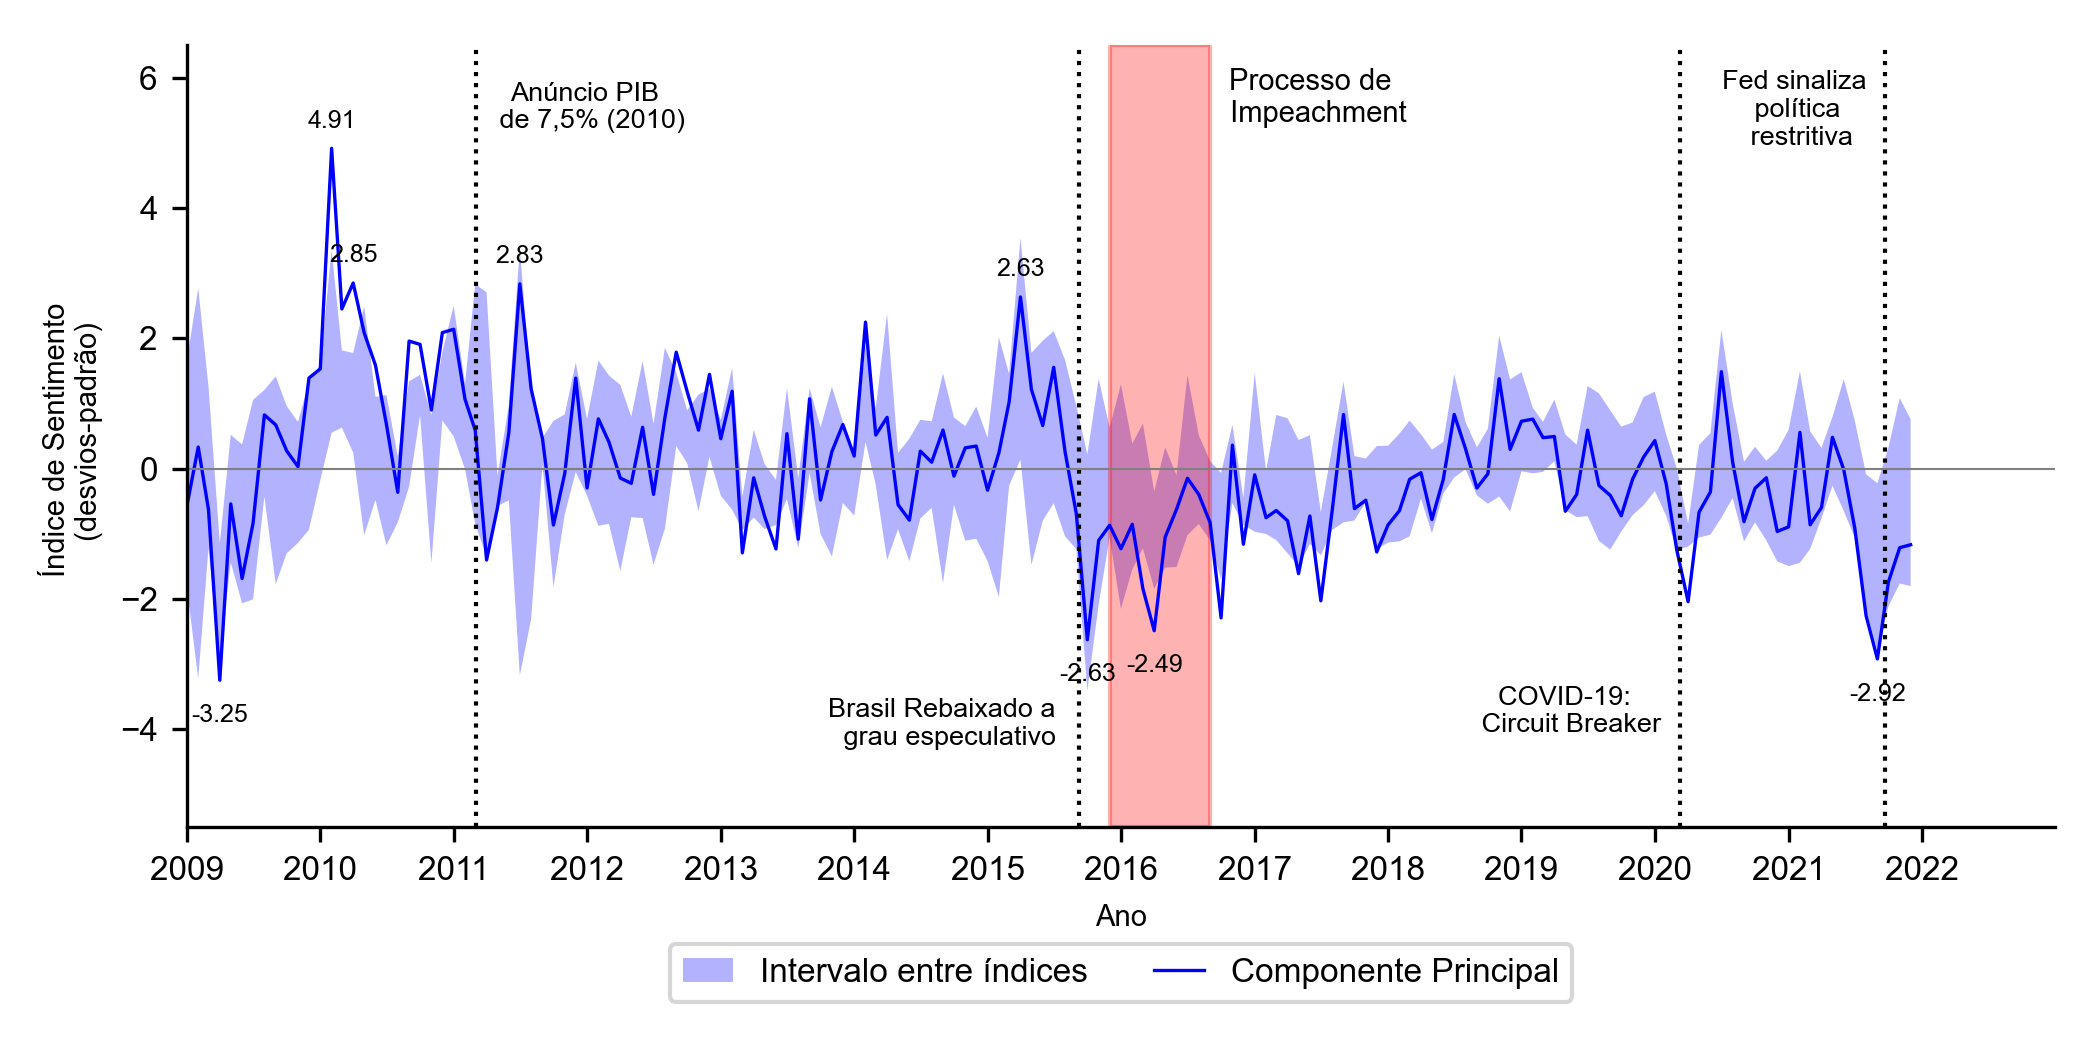
\includegraphics[width=\textwidth]{imagens/pca_plt.png} % Scales the image to fit within margins
    \label{graf:pca}
    \par\noindent
    \begin{minipage}{\textwidth}
        \centering
        \footnotesize % Adjust font size if needed
        \textit{Fonte: Elaboração Própria}
    \end{minipage}
\end{figure}

Da Figura \ref{graf:pca} é possível depreender a existência de dois regimes de comportamento do Componente Principal de forma que até 2016, os valores do índice de sentimento tendem a variar acima da média. Após esse período, a maior parte dos valores varia abaixo média. Além disso, os quatro picos com valores máximos estão localizados antes de 2016 e três picos com valores mínimos após esse ano. Se o valor do Componente Principal sintetiza a variação dos índices de sentimento, então é possível estender essa interpretação ao comportamento dos índices de forma individual.

É bem conhecida a deterioração do cenário político e econômico durante os anos de 2015 e 2016, onde o PIB caiu 3,5\% e 3,3\% respectivamente. Além disso, a inflação, mensurada pelo IPCA, atingiu 10,67\% em 2015, o maior valor da série desde 2002, forçando uma política monetária mais restritiva. 

De um modo geral, a evolução do Componente Principal dos índices de sentimento dialoga com importantes eventos econômicos e apresenta comportamento esperado durante certos intervalos. Esses resultados apontam para a utilização tanto dos índices particulares quanto do próprio componente principal que pode atuar como uma \textit{proxy} do comportamento de variação dos diversos índices. 

\clearpage

\section{Modelos}

Os modelos VAR e \textit{Local Projections} foram construídos segundo o ordenamento de variáveis proposto pela matriz \(B_0\), página \pageref{matrix:matriz_b_ordenamento}. Foram testados todos os oito índices de sentimento produzidos, bem como os dois componentes principais gerados a partir das duas fórmulas de agregação de sentimento. 

Para conferir robustez à modelagem foi aplicada uma ampla gama de variações em termos de transformação das variáveis, técnicas de estacionarização, escolha da ordem \(P\) de autoregressividade dos modelos, bem como foram promovidos novos ordenamentos na matriz \(B_0\) e mesmo inclusão ou exclusão de algumas variáveis. 

O melhor modelo obtido, levando em consideração como critério de julgamento a obtenção de significância estatística dos coeficientes estimados, foi aquele cujo índice de sentimento se fundamenta no dicionário SentiLex e na fórmula de agregação de \textcite{carosia_analyzing_2020}. As variáveis e o ordenamento da matriz \(B_0\) é exatamente o apresentado na seção \ref{metodologia_series_temporais}. As variáveis foram tomadas em nível com aplicação da transformação logarítmica seguindo o tratamento apresentado pela maior parte da literatura na Tabela \ref{tab:var_trabalhos_nacionais}. Adicionalmente, foi aplicado o filtro de sazonalidade X13-ARIMA-SEATS nas variáveis. A escolha da ordem do modelo foi realizada de acordo com o critério de informação AIC, que sugeriu a implementação de quatro \textit{lags} temporais. Todas as raízes do polinômio característico se encontram dentro do círculo unitário, confirmando a estabilidade do modelo. Inicialmente, todos as especificações foram construídas segundo o modelo VAR de forma a estabelecer uma conexão com a literatura nacional. Posteriormente, foram estendidas à modelagem \textit{Local Projections} de forma que pudessem ser geradas comparações entre as duas estratégias de modelagem. 

A Figura \ref{graf:lp_var_comparison} apresenta um comparativo das FRI geradas tanto pelo modelo VAR quanto pelo modelo \textit{Local Projections} segundo as especificações anteriormente definidas. As FRI representam as respostas dinâmicas de cada variável a um choque positivo de um desvio-padrão no termo de erro da variável de sentimento da política monetária. 

\begin{figure}[H]
    \captionsetup{position=above} % Coloca a legenda acima da imagem
    \caption{Funções de Impulso Resposta à um choque na variável de sentimento}
    \centering
    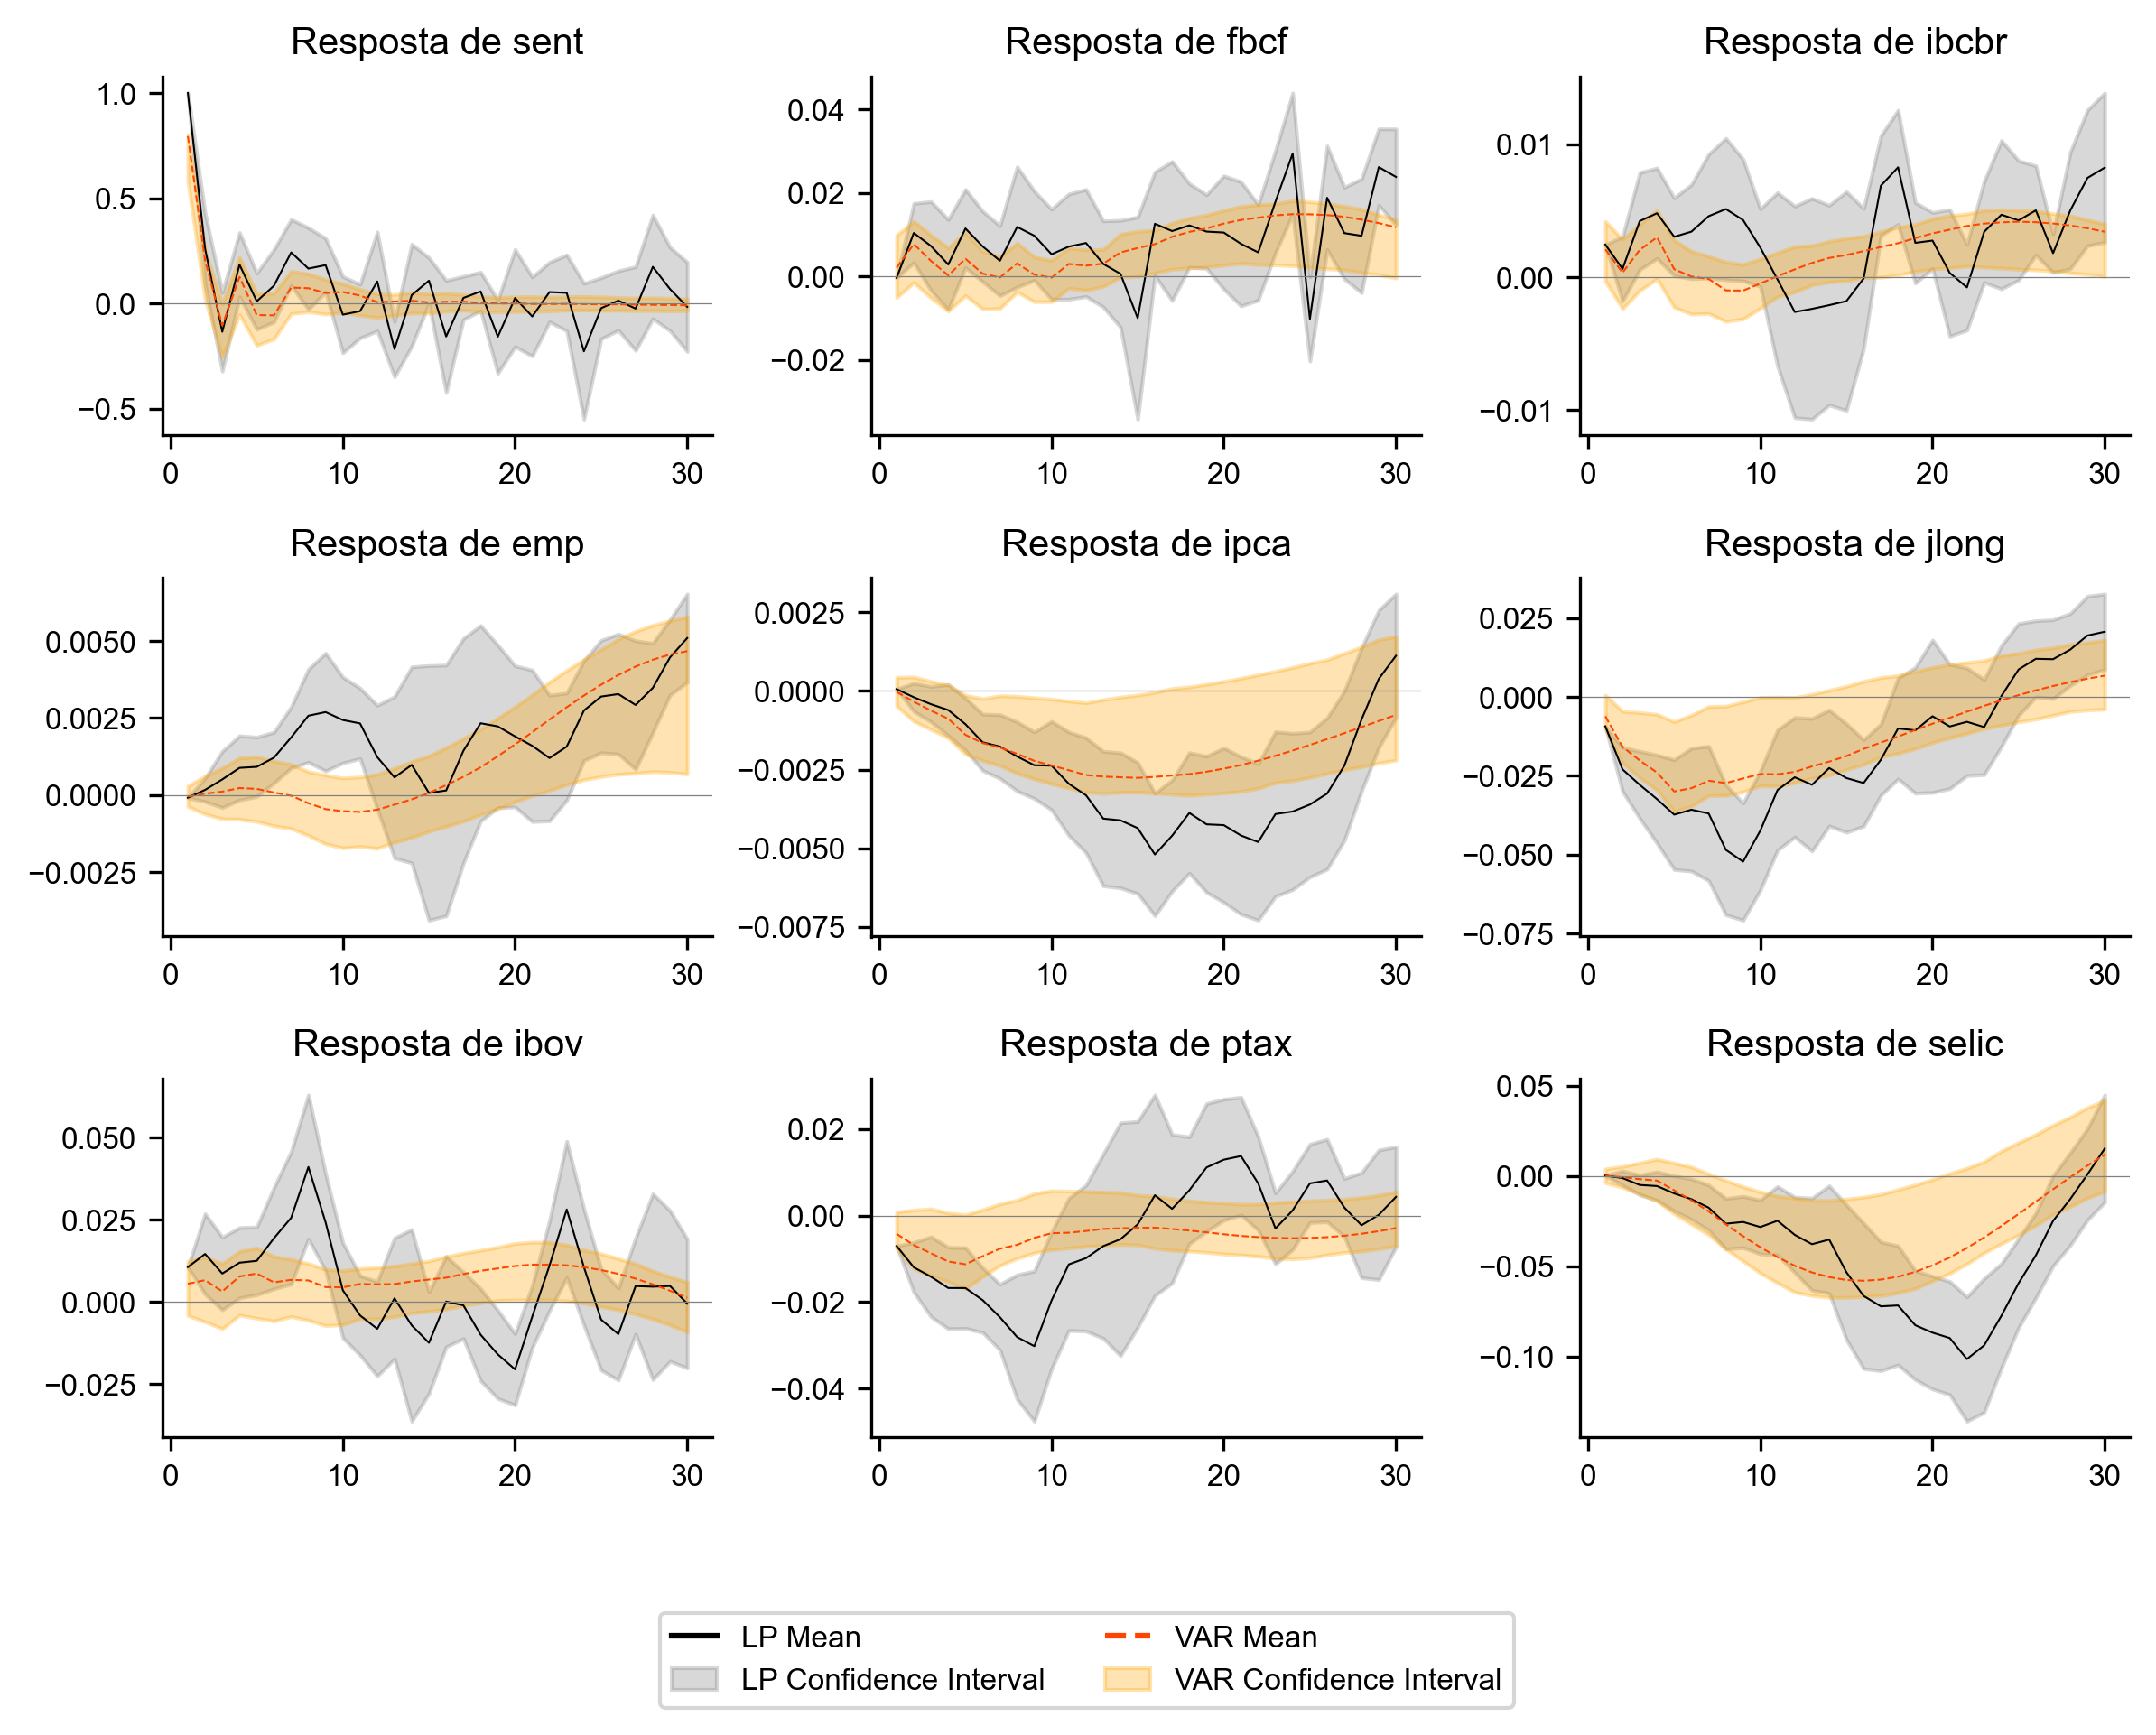
\includegraphics[width=\textwidth]{imagens/lp_var_comparison.png} % Adjust to fit within margins
    \label{graf:lp_var_comparison}
    \par\noindent
    \begin{minipage}{\textwidth}
        \centering
        \footnotesize % Adjust font size if needed
        \textit{Fonte: Elaboração Própria}
    \end{minipage}
\end{figure}

É possível depreender da Figura \ref{graf:lp_var_comparison} uma convergência entre os modelos VAR e \textit{Local Projections} no que se refere ao sentido do efeito das variáveis, especialmente as financeiras. Assim sendo, um choque positivo de um desvio-padrão na variável de sentimento da política monetária causa uma queda estatisticamente significante do IPCA entre quatro e quinze meses nos dois modelos. Essa queda se estende por um horizonte maior no modelo \textit{Local Projections} e com magnitude mais acentuada.

Uma resposta mais imediata ao choque positivo no sentimento ocorre com a variável de juros de longo prazo (jlong). Por ser uma variável tipicamente financeira, trata-se de um resultado esperado. Também para essa variável ambos os modelos apontam em um sentido comum do efeito: um choque positivo no sentimento diminui os juros de longo prazo com magnitude maior para o modelo de \textit{Local Projections} do que para o modelo VAR.

A Selic segue comportamento semelhante as taxas de juros de longo prazo, porém com efeito retardado. Trata-se de um resultado alinhado com a teoria, uma vez que a diminuição das taxas de juros de longo prazo reduz a inclinação da curva de juros, possibilitando margem de manobra para operação da taxa básica de juros. 

As outras duas variáveis financeiras, índice IBOVESPA (ibov) e o câmbio (ptax), apresentam resultados esperados e significativos para o modelo \textit{Local Projections}, mas não para o modelo VAR. Assim, um choque positivo na variável de sentimento da política monetária leva à uma valorização da bolsa de valores no primeiro caso e uma apreciação cambial no segundo. 

As variáveis reais apresentam um resultado mais intrigante. Tanto a FBCF, quanto o IBC-BR e o nível de emprego apresentam uma resposta positiva ao choque na variável de sentimento pelos dois modelos, contudo restritas a um prazo extenso. No modelo VAR, os coeficientes apenas são significativos após quinze ou vinte meses. O modelo \textit{Local Projections} apresenta significância em alguns intervalos antes desse período, mas não de forma consistente. Trata-se de um resultado que necessita de maior investigação para sua clareza, uma vez que pode indicar uma reação do setor real da economia a um choque positivo na política monetária \textit{ceteris paribus}, ou seja, já considerados os efeitos de variáveis financeiras importantes, tal como os juros de longo prazo. 





\bigskip